% % % Headers and definitions
\documentclass[11pt,letter]{article}
\usepackage{times}
           
%\usepackage{mathtools}
\usepackage{float}

\usepackage[left=1.5in,right=1in,top=1in,bottom=1in]{geometry}

%\usepackage[margin=1in]{geometry}
%\usepackage{fullpage} % sets more standardized margins
\usepackage{graphicx} % some graphics functions I use 
\usepackage{abstract} % abstract function
\usepackage{gensymb}
\usepackage{xcolor}
\usepackage[final]{pdfpages}
\usepackage[english]{babel}
\usepackage{blindtext}
\usepackage{pdfpages}
\usepackage{biblatex}

%\usepackage [english]{babel}
\usepackage [autostyle, english = american]{csquotes}
\MakeOuterQuote{"}

\setlength{\parskip}{1em} % The \par command now skips a line between paragraphs, eliminates warnings from using the \par or \\ commands
\setlength{\parindent}{0em} % Left justifies paragraphs after a \par command 
\renewcommand{\baselinestretch}{1.5}

%\addtolength{\textheight}{1in}

\stepcounter{secnumdepth}
\stepcounter{tocdepth}

\renewcommand{\absnamepos}{flushleft} % left justifies abstract
\setlength{\absleftindent}{0pt}
\setlength{\absrightindent}{0pt}

%\onehalfspacing
\begin{document}

\begin{titlepage}

\pagenumbering{gobble}

% Title and author
%\title{  \textbf{ECLECTIC} \\ 
%ECE 403 Final Report}
%\author{Bailee Bartash, Electrical Engineering\\
%  	Cameron Newland, Electrical Engineering}
%\date{\today}

	\centering
	{\scshape\LARGE University of Maine \par}
	\vspace{0.5cm}
	{\scshape\LARGE Electrical Engineering \\ Senior Project Design Report\par}
	\vspace{2.5cm}
	{\Huge EnCLosure for Electronic Component Testing of Integrated Circuits \\ (ECLECTIC)\par}
	\vspace{2.5cm}
	{\Large\itshape Bailee Bartash, Electrical Engineering \\
	Cameron Newland, Electrical Engineering \par}

	\vfill

% Bottom of the page
	{\large \today\par}

\end{titlepage}

\newpage

%\frontmatter
\pagenumbering{roman}
% % % % % % % % % % % % % % %		
% Abstract 
\begin{abstract}
% REWRITE
An environmental chamber for testing the effects of temperature variation on electronic circuits was designed, built, and tested. A CP60333 Peltier module controls the temperature within the chamber to be above and below 300K. A temperature sensing device, in this case the TMP36 integrated circuit (IC), was placed within the chamber. The sensed temperature within the chamber was displayed on the liquid crystal display (LCD) of an STM32L4 discovery board. The desired temperature was set using a joystick on the same discovery board to increment or decrement. The project was externally powered by 120V$_{rms}$ from a wall outlet, which was stepped down using a MEAN WELL power supply and a LM2575 buck converter. The design specifications were to have a chamber that could be cooled to 0$\degree$C and heated to 50$\degree$C, with a temperature measurement accuracy of $\pm$2$\degree$C. The Peltier module also had to be capable of driving at least 2A of current. All of these specifications, as well as the the input and output specifications for a user input and digital representation of the sensed temperature, were met with the final project.  
\end{abstract}

% % % % % % % % % % % % % % % 
% Tables of contents, figures, tables, acronyms, etc
\newpage % jumps to new page
\tableofcontents

\newpage
\listoffigures

\newpage 
\clearpage


\pagenumbering{arabic} % Turn on page numbering

% % % % % % % % % % % % % % %
% Introduction section
\section{Introduction}
This report describes the design and construction of a temperature controlled environmental testing chamber for electronic components. In electronics, there are two general types of devices: passive and active. Passive devices include resistors, capacitors, and inductors. Active devices are semiconductor-based components, such as transistors, op-amps, and microcontrollers. The performance characteristics of these components and the circuits that contain them are highly temperature dependent. This phenomenon is a valuable demonstration in learning about electronics. In everyday settings, temperatures can deviate considerably from the standard operating temperature (300K or 27$\degree$C). A small environmental chamber which can be heated above or cooled below room temperature was designed for the testing of electronic circuits with active compnoents. 

A Peltier module is an active heat pump that can both heat and cool and thus can be a temperature controller. It works by moving electrons to one side of the device, creating a temperature gradient, when supplied with power. Which physical side of the Peltier device is the hot side and the cool side can be changed if the direction of the current flowing through the module is changed. This was achieved in this project using an H-bridge and appropriate gate drivers. The desired temperature is set using the joystick on an STM32L4 discovery board and a temperature sensing IC inside the chamber relays the measured temperature. Both temperatures are displayed on the discovery board LCD. If the temperature set and sensed are different, one pin on the discovery board is set high for the appropriate direction of the current. The project is externally powered by 120V$_{rms}$, and a power supply and a buck converter power the components of the chamber.  

Three specifications are stated in the contract (see Appendix A): the temperature within the chamber needs to be variable, the minimum range is 0-50$\degree$C, with measurable accuracy within $\pm$2$\degree$C, and the driver to the Peltier device needed to be capable of driving a minimum current of 2A. The temperature specification was verified by using a sensor that has an accuracy specification within 1$\degree$C. The accuracy of the sensor was confirmed by using an infrared (IR) thermometer. The current specification was verified by breaking the circuit at the input to the Peltier device and using an unfused multimeter. The inputs to the project are 120V$_{rms}$ from a standard wall outlet and a user control to set the temperature. The output of the project is a digital representation of the temperatures.   

This project was built for classroom applications to test small ICs. Other environmental chambers used to test electronic components are larger and meant for industry, not comparing the behavior of lab components to show the effect of temperature on semiconductors. 

The project is explored further in the following sections of this report. Section 2 is a high-level overview. Section 3 provides design choices and in-depth details. Section 4 gives the measurable results of the project, and Section 5 concludes the report.
% % % % % % % % % % % % % % %
% Breakdown
\section{Breakdown} % Bailee 
This section breaks the project down into four functional blocks for an overview. The goal of this project was to develop a temperature controlled chamber in which electronic ICs can be tested for an observer to note the variations in the behavior of semiconductor based components as a function of temperature. The four blocks are shown in Figure~\ref{fig:blockdiagram}, the high-level block diagram.

\begin{figure}[H]
    \centering
    \includegraphics[width=0.8\textwidth]{blockdiagram.png}
    \caption{Block diagram of ECLECTIC.}
    \label{fig:blockdiagram}
\end{figure}

Starting in the upper left-hand corner of the block diagram and moving to the right and down, "Mains Power" is provided to the project from a standard American wall outlet. This 120V$_{rms}$ signal goes through the "Power Management" block and results in two stepped-down voltages, 12V$_{DC}$ and 5V$_{DC}$. The gate driver, H-bridge, and the external DC fan use 12V$_{DC}$ as a power supply. 5V$_{DC}$ powers the temperature sensor and the temperature control block. The temperature control block also requires an input of a user-selected temperature and measures the temperature within the thermoelectric chamber, displaying both on an LCD display. After the microcontroller of the temperature control unit compares the two temperatures and determines whether the chamber needs to be heated or cooled, the appropriate pin is set and a corresponding signal proceeds through the gate driver and H-bridge to set the current of the Peltier module in the chamber to a specific direction. The chamber houses the Peltier module to heat or cool, a fan to keep the outside of the Peltier module room temperature, and heat sinks to improve the heat transfer. The full schematic of ECLECTIC is provided below in Appendix B.

\subsection{Power Management} % Cam

As specified by the contract, the project is powered by 120V$_{rms}$ (a standard wall outlet), which is the input to the power management block. The power management block converts 120V$_{rms}$ to 12V$_{DC}$ and 5V$_{DC}$. The gate driver, H-bridge, and DC fan are powered with the 12V$_{DC}$ supply and the temperature control block and temperature sensor are powered with the 5V$_{DC}$ supply. A MEAN WELL power supply steps the voltage down to 12V$_{DC}$; whereas a buck converter circuit uses a 12V$_{DC}$ input to produce a 5V$_{DC}$ output.

\subsection{Temperature Control} % Bailee

The temperature control block provides the information signal for the project. An STM32L4 discovery board constitutes most of the temperature control block, which is where the user will input a desired temperature and read that and the measured temperature. A feedback loop from a temperature sensor located inside the chamber is an input to the temperature control. The measured temperature is compared to the user temperature and the discovery board will set one GPIO pin high if the chamber needs to be heated and another GPIO pin high if it needs to be cooled. Then, a PWM generator and an analog logic circuit will provide the input signals to the gate driver.

\subsection{Gate Driver $\&$ H-Bridge} % Cam

The driving force behind switching the direction of the current through the Peltier device is a MOSFET-based H-bridge, which requires a gate driver. Depending on the signal from the temperature control block, the gate driver and H-bridge electronically switch the direction of the current to either cool or heat the chamber. Both subcircuits use a 12V$_{DC}$ power supply. The inputs are four individual signals from the temperature control block to produce gate signals with the ability to turn on the MOSFETs. The orientation of the conducting MOSFETs produces the direction of the current necessary to cool or heat the chamber.

\subsection{Thermoelectric Chamber} % Bailee

The thermoelectric chamber is a physical box made out of insulating foam board in which the semiconductor IC is placed. This chamber is relatively small, 4" wide by 4" long and 2.5" tall, in order to meet the temperature range specification. Several components are located within the thermoelectric chamber. The main component, and the basis for this overall project, is a Peltier module, which takes in the current as supplied by the H-bridge and will heat or cool depending on the direction of that current. Two heat sinks and a DC fan are also included in the chamber to properly disperse the heated or cooled air. The temperature sensor is also located within the chamber. 


% % % % % % % % % % % % % % %		
% Details
\section{Details}

The design, test, and construction of ECLECTIC are discussed in this section. The design is built on work in previous courses, especially Electronic Power Conversion and Microcomputer Architecture and Applications. The hardware of the project can be traced through the functional blocks of the block diagram shown in Section 2. The software of the project provides the signals for setting and changing the chamber temperature. The details provide further explanation of the project modules described in the breakdown. Section 3.1 discusses is power management, followed by Section 3.2, temperature control, Section 3.3, gate drivers $\&$ H-bridge, and Section 3.4, the thermoelectric cooler. The full schematic for ECLECTIC is given in Appendix B and the parts list is given in Appendix C. 

\subsection{Power Management}

The project is powered with a 120V$_{rms}$ standard wall outlet. The power management block converts this supply to 12V$_{DC}$ and 5V$_{DC}$ to power all the components of the project.

\subsubsection{MEAN WELL Power Supply}

The purpose of the MEAN WELL power supply is produce the 12V$_{DC}$ voltage supply necessary to power the entire circuit. The power supply was chosen with a power rating beyond the scope of the project to allow design flexibility.

The MEAN WELL power supply is a 150W supply, where the output is a 12V$_{DC}$ voltage with the ability to handle up to 12.5A of current. This became useful when calibrating the project to drive more current to reach the extreme temperature specifications. This output voltage is necessary primarily for the buck converter, the 12V$_{DC}$ fan, and the gate drivers and H-bridge. Another useful feature was the provision of two rails that could provide 12$_{DC}$. This MEAN WELL power supply was purchased directly from Digi-Key.

\subsubsection{Buck Converter}

The low power elements of the project required a 5V$_{DC}$ input. The most efficient method to step down a DC voltage was by using a buck converter. Buck converters are switched-mode regulators, which are a newer class of power supplies that are less bulky and generally better for high-frequency applications than their predecessors, linear power supplies. Switched-mode regulators, and by extension buck converters, are preferable for some applications over linear power supplies as they are more efficient, having only two states: on or off. A buck converter achieves the stepped down voltage without dissipating the excess voltage via heat loss, an advantage over a linear regulator, which is the linear power supply version of the buck converter. 

A buck converter operates with a transistor acting as a switch at a specific duty cycle convert the higher input voltage to the lower output voltage. The inductor is used to provide constant current to the load, the capacitor is used to smooth the output voltage, and a Schottky diode allows the transistor to turn on and off freely by creating another path for current. The LM2575T buck IC was used to convert this voltage supply in this project. The circuit schematic for this IC as well as the component values of the final circuit are shown below in Figure \ref{fig:buck}.

\begin{figure}[H]
    \centering
    \includegraphics[width=0.7\textwidth]{Buck.png}
    \caption{Schematic for the LM2575 buck converter.}
    \label{fig:buck}
\end{figure}

The initial value to find for this design was the duty cycle of the transistor so that the inductor value can be solved. The equation from \textit{Power Electronics} [1]
\begin{equation}
    V_o = V_s*D
\end{equation}

where a V$_O$ of 5V and V$_S$ of 12V resulted with a duty cycle D of $\frac{5}{12}$, or 41.67$\%$. The equivalent resistance was also needed for the load of this circuit. The current draw was estimated to be 100mA at 5V, so the equivalent resistance was estimated to be 50$\Omega$. From this, the equation

\begin{equation}
    L1_{min} = \frac{(1-D)*R}{2*f}
\end{equation}

also from \textit{Power Electronics} was used to solve for the minimum inductor value of the buck converter to ensure constant current where $f$ was the oscillator of the buck converter was 52kHz. From this, the calculated inductor minimum was found to be 330$\mu$H and chosen to be 1000$\mu$H to ensure a constant current to the load.

The SB120 Schottky diode was chosen primarily because of its use as a barrier and fast frequency switching operations. The reason for the diode in this circuit is to allow another path of current to flow when the transistor switches off since the current through the inductor cannot change instantaneously. The low voltage drop across the diode was also desirable to prevent unnecessary power losses.

The capacitor values, especially the one at the output, assumes a desired ripple of the output voltage so that the capacitor value could be solved. For this design, the ripple was chosen to be very small since this supply was used to power the discovery board. So, the ripple was chosen to be 0.05$\%$. From \textit{Power Electronics} [1], the equation
\begin{equation}
    C12 = \frac{1-D}{8*L1*\frac{\Delta V_o}{V_o}*f^2}
\end{equation}

was used where $\frac{\Delta V_o}{V_o}$is 0.0005. 

From this, the calculated capacitor value was 164$\mu$F, so the chosen capacitor value was 470$\mu$F to decrease the ripple further.

This signal was the 5V$_{DC}$ as required by the discovery board, as mentioned before. It was important to make sure this supply was clean as possible because it was used for the PWM signals for the gate drivers after being passed through the rest of the temperature control block, as explained in Section 3.2 and Section 3.3. 

\subsection{Temperature Control}

The temperature control portion of this project is the main signal generator. Within this module, the desired temperature was is set, the temperature from inside the chamber is measured, and whether the chamber needed to be heated or cooled is determined. The temperature control block consists of a temperature sensor, the microcontroller of the STM32L4 discovery board, a PWM generator, and a logic circuit.

\subsubsection{Temperature Sensor}

The temperature sensor required for this project is located inside the environmental chamber. It takes the temperature of the chamber and relays the measurement back to the microcontroller of the project. This measurement is critical as it is the means of comparison for the user-specified temperature and determines whether the chamber needs to be heated or cooled. Many varieties of temperature sensors exist, and the temperature sensor chosen is a sensor IC. The particular sensor IC selected is the TMP36. 

The operating temperature range and the temperature sensing range for the TMP36 is greater than typical ICs at -40$\degree$C to 125$\degree$C. With sensor ICs, the temperature can be measured continuously and read at any time. The accuracy of the sensor is rated to be within $\pm$0.5$\degree$C of the actual temperature. Temperature sensors of the TMP36 variety are typically powered by a 5V supply and the output voltage is linearly related to the temperature in Celsius, where an increase of 10mV in the output corresponds to one degree Celsius rise in temperature. The TMP36 was also desirable because it has an offset of 500mV, and this protects the ADC from incorrectly reading temperatures close to 0$\degree$C. This means that the output of the TMP36 would be anywhere between 500mV and 1V, and these voltages would correspond to 0$\degree$C and 50$\degree$C, respectively. For example, if the output voltage was 627mV, the sensed temperature would be approximately 12.7$\degree$C.

The TMP36 has a power rail (which can be between 2.7V and 5.5V), ground, and V$_{out}$, where the output is read. The pin layout for the TMP36 and its related sensors is shown in Figure~\ref{fig:tempsensor}.

\begin{figure}[H]
    \centering
    \includegraphics[width=0.3\textwidth]{tmp36.JPG}
    \caption{Wiring diagram for temperature sensor.}
    \label{fig:tempsensor}
\end{figure}

The TMP36 does not have the shutdown pin from Figure~\ref{fig:tempsensor}. This sensor IC was also a practical choice as it was straightforward to interface to a microprocessor. An on-board ADC polls the pin connected to the temperature sensor through the pin PA1 on a STM32L4 discovery board. More detail on the microprocessor and the discovery board are provided in Section 3.2.2.

\subsubsection{STM32L4 Discovery Board}

For this project, a microprocessor was required in order to compare the user-specified temperature to the measured temperature of the chamber and then provide a response to heat or cool the chamber. The software of the project is contained within the microprocessor. As other components were also required, including an analog to digital converter (ADC), to read the temperature from a sensor, some general purpose input-output (GPIO) pins, to send the appropriate signal to the rest of the temperature control block, and a display for the temperature, a discovery board was the ideal choice to easily interface with all of the peripherals.

Because the team has used the STM32L4 discovery board in previous courses, it offered some familiarity. It also provided all of the necessary hardware components for the software requirements. Figure~\ref{fig:discovery} below shows the pin layout of the discovery board and the peripherals.

\begin{figure}[H]
    \centering
    \includegraphics[width=0.4\textwidth]{DiscoveryBoard.png}
    \caption{Schematic of the STM32L4 discovery board.}
    \label{fig:discovery}
\end{figure}

As shown on the schematic above and in the block diagram of Figure~\ref{fig:blockdiagram}, the discovery board has three inputs and two outputs. The STM32L4 discovery board requires an input voltage of 5V. During programming and debugging, this supply was provided by a USB port on a PC. When the project was being operated fully, the buck converter provided the 5V. 

The user provides the second input, and this will be discussed in the next section. The third input is the output voltage from the temperature sensor, which corresponds to the expected sensed temperature between 0 and 50$\degree$C. This input, as described above, is polled by an on-board ADC and pin PA1, and the rail and ground required by the sensor is also provided by the discovery board. 

From the contract specifications, one of the outputs of the project must be a digital representation of the sensed temperature. This is detailed in Section 3.2.3.3. The other output of the discovery board is a signal directed from the GPIO pin (PE14 or PE15) to the PWM generator to produce the appropriate current to power the Peltier device of the thermoelectric chamber. More details are given in Section 3.2.2.2 and in Section 3.2. The datasheet for the STM32L4 discovery board is referenced below [2].

\paragraph{User Input} \

The main input of the temperature control block is a user input that sets the desired chamber temperature. The temperature range of the chamber should be between 0-50$\degree$C. This means that the user should be able to set any temperature within 0-50$\degree$C. The increment and decrement scales were set to be integers for the $\pm$2$\degree$C accuracy specification. The joystick on the discovery board was used was used to set the temperature. Figure~\ref{fig:joystick} below shows the wiring diagram for the joystick.

\begin{figure}[H]
    \centering
    \includegraphics[width=0.8\textwidth]{joystick.JPG}
    \caption{Wiring diagram for the STM32L4 discovery board joystick [2].}
    \label{fig:joystick}
\end{figure}

As shown in Figure~\ref{fig:joystick}, each portion of the joystick corresponds to an input-output pin on the discovery board. Excluding the left arrow, each part of the joystick is available for the user input. PA1 also corresponds to the on-board ADC used to poll the temperature sensor, the connection between that pin and the joystick was removed by removing the 0$\Omega$ resistor, shown on the wiring diagram. 

The other sides of the joystick (up, down, right, and center) were configured to correspond to changes in the set temperature. The original set temperature was initialized to 23$\degree$C, as this is room temperature. An interrupt handler was configured using the program STM32Cube, and the pin corresponding to each portion of the joystick was set to increment or decrement this set value. 

For convenience, the up and down portions of the joystick increment and decrement the set temperature by 1$\degree$C, respectively. As there is a wide range of temperatures that the chamber temperature should be able to be set to, the right portion of the joystick was set to increment the temperature by 10, being capped at a set temperature of 50$\degree$C, and the center portion of the joystick was set to decrement the temperature by 10, capped at 0$\degree$C.

\paragraph{Temperature Comparison} \

The means of temperature comparison to determine whether the chamber required heating or cooling is straightforward. The two temperatures, the set temperature from the user input and the measured temperature from the sensor output, were assigned to variables in the main function of the code. In three for loops, they were compared to determine whether or not the set temperature was different from the measured temperature. If there was a difference, the comparison algorithm then determined whether the set temperature was greater than the measured temperature or less, and then the appropriate GPIO pin on the discovery board, as discussed in Section 3.2.2.1, was set or reset. Figure~\ref{fig:software} below shows the software flow of the temperature comparison. 

\begin{figure}[H]
    \centering
    \includegraphics[width=0.45\textwidth]{SoftwareFlow.png}
    \caption{Software algorithm for the temperature comparison.}
    \label{fig:software}
\end{figure}

As shown on Figure~\ref{fig:software} above, if the set and measured temperature are the same as or very close to each other, both the HEAT and COOL pins are reset. If the set temperature is greater than the measured temperature, the HEAT pin is set, COOL is reset. If the set temperature is less than the measured temperature, the COOL pin is set, HEAT is reset. The GPIO pin provides the signal to the PWM generator and varies the input to the logic circuit, and eventually, the direction of the current through the Peltier device. This signal flow is explained further in Section 3.2.4 and Section 3.3.

\paragraph{LCD Display} \

The STM32L4 discovery board has a liquid crystal display (LCD) on the front of the board that is capable of displaying six characters. For this project, the set temperature, significant to the ones digit and the tens digit, is displayed on the right side of the LCD and the measured temperature, with the same layout, is displayed on the left side of the LCD. There is space for two characters between these numbers to help with distinction between the two.

PE14, the COOL pin, is connected to a blue LED. PE15, the HEAT pin, is connected to a red LED. When a pin is set because the chamber is heating or cooling, the corresponding LED is lit. If neither LED is lit the set temperature should match the measured temperature.

Figure~\ref{fig:BLUE} and Figure~\ref{fig:RED} show the STM32L4 discovery board cooling and heating, respectively. 

\begin{figure}[H]
    \centering
    \begin{minipage}{0.5\textwidth}
        \centering
        \includegraphics[width=0.65\textwidth]{BLUEBoard.jpg} % first figure itself
        \caption{Chamber in cooling mode.}
        \label{fig:BLUE}
    \end{minipage}\hfill
    \begin{minipage}{0.5\textwidth}
        \centering
        \includegraphics[width=0.65\textwidth]{REDBoard.jpg} % second figure itself
        \caption{Chamber in heating mode.}
        \label{fig:RED}
    \end{minipage}
\end{figure}

In order to develop this display, the main function of the code required the same variables as the temperature comparison algorithm. Four 8-bit integers were declared for the four digits of the set temperature and the measured temperature. For the measured temperature, the input signal as seen by the discovery board was a voltage between 0V and 500mV, which appeared in hexidecimal correctly but required scaling to be seen in decimal correctly. This scale was determined by considering the input voltage to the microprocessor on the discovery board, 3.3V, and the number of bits, 10. This value was then divided by 10 for an integer value like the set temperature, doable because of the linearity between the output voltage of the temperature sensor and the actual measured temperature.

The set value and the measured value were both divided by 10 to find the tens digit of the temperature to be displayed. These were assigned to display on position 0 and position 4, respectively. The two temperatures were then analyzed having taken modulo 10, which results in the remainder as the number is divided by 10, giving the ones digit of the temperature to be displayed. These were assigned to display on postion 1 and position 5 of the LCD, respectively. 

\subsubsection{PWM Generator}

The PWM generator uses a 555 timer circuit to create a  75.3$\%$ duty cycle rectangular wave with a 7.14kHz frequency. It is used to create four individual signals for the gate driver circuits explained further in Section 3.2.4. An exact frequency value is not as important to design as the duty cycle. It must be between two extremes because of the gate driver ICs and the size of the bootstrap capacitor. The two diode circuit improves the design and was used in the final circuit.

If the frequency from the 555 timer is too fast, then the bootstrap capacitor lacks the time to charge up to its appropriate value. And, if the frequency is too slow, then the gate voltage for the MOSFET will drop as the capacitor drains. Therefore, a frequency around 10kHz works well. The design for the PWM generator by using a 555 timer is illustrated below in Figure~\ref{fig:PWM}.

\begin{figure}[H]
    \centering
    \includegraphics[width=0.7\textwidth]{PWM.png}
    \caption{Schematic PWM generator.}
    \label{fig:PWM}
\end{figure}

The sizing of C5, R2, and R3 determine the frequency and duty cycle of the PWM output signal. The duty cycle for the 555 timer is the most important, so choosing the values for the two resistors is first. The rise time and total time of the signal are given by
\begin{equation}
    T_1 = ln(2)*R2*C5
\end{equation}
and
\begin{equation}
     T_2 = ln(2)(R2+R3)*C5
\end{equation}
so from [3] the duty cycle can be simplified to
\begin{equation}
    Duty = \frac{R2}{R2+R3}.
\end{equation}

This source used to help the team understand the improved circuit became more useful because if a duty cycle of 75$\%$ is desired, only two parameters are needed. R2 is chosen to be 3.3k$\Omega$ and R3 is chosen to be 1k$\Omega$ for a calculated 75$\%$ duty cycle. A large frequency range is allowed for the gate driver IC signals, so the nearest available capacitor value from the one calculated worked just as well. The equation

\begin{equation}
    f = \frac{1}{ln(2)(2R2+R3)*C5}
\end{equation}

from [3] is rewritten as 
\begin{equation}
    C5 = \frac{1}{ln(2)(2R2+R3)*f}
\end{equation}

where the frequency is chosen to be 10kHz as a starting point to see the relative value of C5. From this, a capacitor value of 31nF is calculated so a 33nF capacitor is chosen as the closest value readily available. Using these values, the PWM generator was built and Figure~\ref{fig:555} below is the output.

\begin{figure}[H]
    \centering
    \includegraphics[width=0.75\textwidth]{555Out.png}
    \caption{Output of the PWM generator.}
    \label{fig:555}
\end{figure}

\subsubsection{AND$/$XOR Gates} %Cam

The AND$/$XOR gates are useful where one 555 timer signal is used to produce four unique signals for the gate driver circuits. The discovery board uses two GPIO pins as control for heating and cooling. Figure~\ref{fig:LogicDiagram} below shows a logic diagram of how the signals are represented under the four conditions of the two GPIO pins.

\begin{figure}[H]
    \centering
    \includegraphics[width=0.41\textwidth]{LogicDiagram.png}
    \caption{Logic diagram.}
    \label{fig:LogicDiagram}
\end{figure}

The logic circuits are used to minimize power loss in the system. The bottom MOSFETs must be the conjugate of the top MOSFETs in order to charge the bootstrap capacitors mentioned in the beginning of Section 3.3.5 below. If M1 and M4 are necessary to produce one direction of current, then M2 is also needed but M3 is not. This is shown in Figure~\ref{fig:HEATCUR} below. 

\begin{figure}[H]
    \centering
    \includegraphics[width=0.41\textwidth]{M1M4CUR.png}
    \caption{Schematic of current flow while heating.}
    \label{fig:HEATCUR}
\end{figure}

By not turning on M3, the current only flows in the direction to heat. The opposite is true where cooling the chamber requires M2 and M3 with M4 the conjugate of the two, but M1 remains off. This is illustrated in Figure~\ref{fig:COOLCUR} below.

\begin{figure}[H]
    \centering
    \includegraphics[width=0.41\textwidth]{M2M3CUR.png}
    \caption{Schematic of current flow while cooling.}
    \label{fig:COOLCUR}
\end{figure}

This again only allows one direction of current that is pulsed at a specific duty cycle so the work that is placed into cooling the chamber is as effective as possible. 

Under the condition where the HEAT pin is on and the COOL is off, M1 and M4 are the same signal, M2 is the conjugate of these two, and M3 is low. The measured signals under the heating condition can be seen below in Figure~\ref{fig:heatLogic}.

\begin{figure}[H]
    \centering
    \includegraphics[width=.7\textwidth]{Heat.jpg}
    \caption{Logic gate outputs while heating.}
    \label{fig:heatLogic}
\end{figure}

The subplots in Figure~\ref{fig:heatLogic} are structured as M1 and M3 in one plot, or the top MOSFET gate signals, and M2 and M4, or the bottom MOSFET gate signals for the gate driver circuit. This is helpful to compare the top signals and bottom signals. Under this condition, M1 and M4 are on and one direction of current is produced with M2 turning on to pulling to node to ground and allow the bootstrap capacitor to charge.

Under the condition where the COOL pin is on and the HEAT is off, M2 and M3 are the same signal, M4 is the conjugate of these two, and M1 is low. The measured signals in this project under the cooling condition can be seen below in Figure~\ref{fig:coolLogic}.

\begin{figure}[H]
    \centering
    \includegraphics[width=.7\textwidth]{Cool.jpg}
    \caption{Logic gate outputs while cooling.}
    \label{fig:coolLogic}
\end{figure}

Again, only one direction of current is permitted when M2 and M3 are on. M4 is still needed to bring the node between the top and bottom MOSFET to ground to charge the bootstrap capacitor, so it is configured as the conjugate of M2 and M3.

When both the HEAT pin and COOL pins from the Discovery Board are off, no current should flow because the chamber is within one degree of the temperature set by the user. So, this condition allows the bottom MOSFETs to pulse at the same duty cycle as the 555 timer. The measurement of this condition can be seen below in Figure~\ref{fig:inSpecLogic}.

\begin{figure}[H]
    \centering
    \includegraphics[width=.7\textwidth]{INSPEC.jpg}
    \caption{Logic gate outputs while within one degree of set temperature.}
    \label{fig:inSpecLogic}
\end{figure}
In Figure~\ref{fig:inSpecLogic}, no current flows as the node between the top and bottom MOSFETs on each side of the Peltier module are pulled to ground when the bottom MOSFETs are turned on. A top MOSFET must conduct and bring the node between the top and bottom MOSFETs to 12V in order to allow a voltage drop across the Peltier device. Since that condition is never met, no current flow is permitted when the HEAT pin and COOL pin are off.

Logic ICs were used to create the four individual signals outlined above in Figure \ref{fig:LogicDiagram}. Figure \ref{fig:logic} below shows the logic IC configuration used to create the appropriate signals for the gate driver and H-bridge circuit.

\begin{figure}[H]
    \centering
    \includegraphics[width=0.8\textwidth]{LogicGates.png}
    \caption{Schematic of logic gates.}
    \label{fig:logic}
\end{figure}

The CD4070 logic gate IC was an XOR gate configuration, so that part of the logic in Figure \ref{fig:LogicDiagram} was able to be implemented directly. The CD4011, however, was a NAND configuration when ANDs were needed, so output of one NAND was tied to the inputs of another NAND to create the appropriate logic configuration.

\subsection{Gate Driver $\&$ H-Bridge}

The gate driver and H-bridge circuit controls the direction of the current through the Peltier module for heating and cooling the chamber. The gate drivers are needed because the logic circuit nor the discovery board can supply enough power to turn on the MOSFETs, especially since the logic circuit is powered from the STM32L4 discovery board. Overcoming the input capacitance of the MOSFET gates is capable with the gate driver ICs externally powered with 12V$_{DC}$. The circuit outlining this task is given below in Figure~\ref{fig:gatedrivers}.

\begin{figure}[H]
    \centering
    \includegraphics[width=1\textwidth]{GateDriver.png}
    \caption{Schematic of gate drivers.}
    \label{fig:gatedrivers}
\end{figure}

Two gate driver circuits are required to have full control over four separate MOSFET gates, so two identical gate driver circuits comprise the gate driver and H-bridge circuit. It is also important to note that the top MOSFETs gates in the H-Bridge need a supply larger than the reference of the H-bridge so that the top MOSFET does not turn off. When the top MOSFET turns on, essentially all of the voltage is dropped across the load. If the source of the top MOSFET has the same voltage as the gate, the V$_{GS}$ is not large enough to keep the MOSFET on. So, the use of a bootstrap capacitor as part of this gate driver circuit allows the gate to be larger than the supply voltage and eliminate this issue. These capacitors are sized according to the frequency of the incoming signals to the gate drivers, provided by the logic circuits, and the required rise/fall time of the gate voltage.

Finally, N-channel MOSFETS were chosen because they have great mobility due to their carriers being electrons. D1 and D2 are provided to allow the 12V supply to charge the capacitors via forward biased diodes. When the top MOSFETs turn on the the BOOST pin is driven to 24V, the diodes are reversed biased to keep the voltage supply 12V.

The gates are measured to show the signals used to turn on the MOSFETs under the heating condition. When heating, M1 and M4 conduct, M2 is the opposite of M1 and M4, and M3 remains off. Figure ~\ref{fig:mosfetgates} below shows these signals measured at the gates of the MOSFETs.

\begin{figure}[H]
    \centering
    \includegraphics[width=.7\textwidth]{MOSFETGates.jpg}
    \caption{MOSFET gate signals while heating.}
    \label{fig:mosfetgates}
\end{figure}

It is clear that M1 and M4 conduct at the same time, but M1 is 24V$_{DC}$, while M4 is 12V$_{DC}$. This is because of the bootstrap capacitor mentioned earlier in this section. The capacitor is referenced to ground when M1 is off and is M2 is on and the capacitor is allowed to charge. As soon as the M2 is turned off and M1 is turned on, the bottom of the capacitor is 12V$_{DC}$ so the top of the capacitor is now 24V$_{DC}$. This is the voltage used to drive M1's gate.

\subsection{Thermoelectric Chamber and its Contents}

The thermoelectric chamber is where the temperature sensitive electronic ICs are placed for testing. The chamber was constructed out of insulated foam board to ensure the internal temperature was maintained. The chamber is a 4 by 4 inch box with a height of 2.5 inces. Although small, these dimensions were required to achieve the project specifications. The foam board was selected to prevent air from dissipating out of the chamber. It is 1 inch thick and has an R value of 5, which corresponds to resistance to heat flow. The higher this value is, the greater the insulation power.

The chamber also houses the temperature sensor, the Peltier device, and one heat sink. Outside the chamber, there is a heatsink/fan combination. The Peltier device and the fans are the key factors to sizing the chamber itself. Moving the air off of the device itself and having a module that can produce the temperature necessary to meet specs was the most important part of specifying these parts. The temperature sensor was previously discussed in Section 3.2.1.

In this project, the previously discussed Peltier device will be placed in the center of the H-bridge so that current control and therefore temperature control can be achieved. The CP60333 Peltier module from CUI Inc. has a maximum current of 6.0A, which provides for a large error margin with the input current to the device, as there is a specification for the MOSFET driver to drive at least 2.0A. The maximum voltage that this device can withstand is 15.4V, one of the highest of available Peltier devices, higher than necessary in order for the device to heat the environmental chamber more efficiently. Lastly, the ability of this device to achieve temperature changes of 66$\degree$C as it deviates from 27$\degree$C exceeds the specification of the temperature range of this chamber.

An external DC fan was required to keep the external side of the Peltier module as close to room temperature as possible. This fan is a critical aspect of the thermoelectric chamber and was selected to be an the Intel E97378 CPU cooler, a fan coupled with a large heat sink. Dispersing room temperature air onto the external side of the Peltier module increases the temperature gradient created by the device and ensures that the internal side of the module is as effective as possible.

On the inside of the chamber, a small heat sink increases the effectiveness of the Peltier device. This small heat sink was provided by the instructor to fit the Peltier device. Thermal paste was used to remove the air insulation and that could possibly occur between the Peltier device and the heat sink to improve effectiveness of the Peltier module.

\section{Results}

Several parameters of the chamber's performance were analyzed to determine whether or not the project met/exceeded the specifications. The range and accuracy of temperature necessary for the chamber were very specific however the accuracy of the displayed temperature was ensured in two ways. 

\subsection{Temperature Range}

One of the most distinct specifications for this project was that the environmental chamber be able to heat up to a temperature of 50$\degree$C and cool down to a temperature of 0$\degree$C. The chamber does meet those two specifications, shown below in Figures \ref{fig:0C} and \ref{fig:50C}. 

\begin{figure}[H]
    \centering
    \begin{minipage}{0.5\textwidth}
        \centering
        \includegraphics[width=0.75\textwidth]{0CSTM.png} % first figure itself
        \caption{ECLECTIC at 0$\degree$C.}
        \label{fig:0C}
    \end{minipage}\hfill
    \begin{minipage}{0.5\textwidth}
        \centering
        \includegraphics[width=0.78\textwidth]{50CSTM.jpg} % second figure itself
        \caption{ECLECTIC at 50$\degree$C.}
        \label{fig:50C}
    \end{minipage}
\end{figure}

The temperatures shown on the LCD were verified with their accuracy in section 4.3 to make sure of the full range could be verified.

\subsection{Driver Current Minimum}

The driver to the Peltier device needed to be capable of driving a minimum of 2A to meet the specification. Calibrating the Peltier device to meet the temperature range specification meant driving the device with more current. The final current through the Peltier device is shown in Figure \ref{fig:current}.

\begin{figure}[H]
    \centering
    \includegraphics[width=0.25\textwidth]{Current.png}
    \caption{Peltier driver current meeting specifications.}
    \label{fig:current}
\end{figure}

An unfused multimeter was utilized to make to make a measurement of 3.54A, well beyond the specification of 2A.

\subsection{Temperature Accuracy}

Temperature accuracy of the displayed measured temperature on the LCD of the discovery board was a significant contract specification. The temperature sensor selected was chosen because it had the smallest possible margin of error at $\pm$0.5$\degree$C. 

The overall temperature accuracy specification was to be within $\pm$2$\degree$C, which provided for flexibility in the project performance and was also the average accuracy rating on several IR thermometers purchased to help verify this specification. In addition to the IR thermometer, an Analog Discovery 2 Digilent was used to measure the output pin of the temperature sensor. The voltage measured corresponds to the temperature sensed. For both measurements, the desired temperature of the chamber was set and the IR thermometer and the Digilent results were recorded. Figure~\ref{fig:comparison} below shows the measured temperature in relation to the set temperature, and the acceptable temperature tolerances.

\begin{figure}[H]
    \centering
    \includegraphics[width=1\textwidth]{untitled.jpg}
    \caption{Temperature readings: expected and measured, with design tolerances.}
    \label{fig:comparison}
\end{figure}

As shown in Figure~\ref{fig:comparison} above, both temperature readings remained within the design tolerances for the entirety of the possible temperature range.

\section{Conclusion}

The project ECLECTIC, the design of ECLECTIC, and the results of testing ECLECTIC have been discussed. The project was built according to design specifications and operated as expected. Several iterations of the project resulted in a temperature-controlled environmental chamber that met the design specifications. The final result required an STM32L4 discovery board, mechanical elements to help the heating/cooling process, and subcircuits designed from previous experience in ECE courses. ECLECTIC can be used as a valuable teaching tool to show students how semiconductor-based integrated circuits may vary in their behavior when operated in temperatures warmer or cooler than room temperature. Operating instructions are provided (Appendix E). 

\begin{thebibliography}{9}
\bibitem{buck}
Daniel W. Hart, \textit{Power Electronics}, McGraw-Hill Comanies, Inc., 2011.

\bibitem{STM}
STMicroelectronics,``Ultra-low-power Arm® Cortex®-M4 32-bit MCU+FPU, 100DMIPS, up to 1MB Flash, 128 KB SRAM, USB OTG FS, LCD, ext. SMPS'' STM32L476xx Datasheet, May. 2015
[Revised May 2018]

\bibitem{55}
Electronic Tutorials, ``555 Oscillator Tutorial,'' April, 2014. [Online] \newline
\textcolor{blue}{\underline{https://www.electronics-tutorials.ws/waveforms/555$\_$oscillator.html}} \newline
[Accessed Oct.13,2018]
\end{thebibliography}

\newpage


% % % % % % % % % % % % % % %		
% Appendices

\appendix

\section*{Appendices}

\section{Appendix: Project Contract}

\begin{figure}[H]
    \centering
    \includegraphics[width=1\textwidth]{contract.jpg}
\end{figure}

\section{Appendix: Schematic}
\begin{figure}[H]
    \centering
    \includegraphics[width=1\textwidth]{Schematic.png}
\end{figure}

\section{Appendix: Parts List}

\begin{figure}[H]
    \centering
    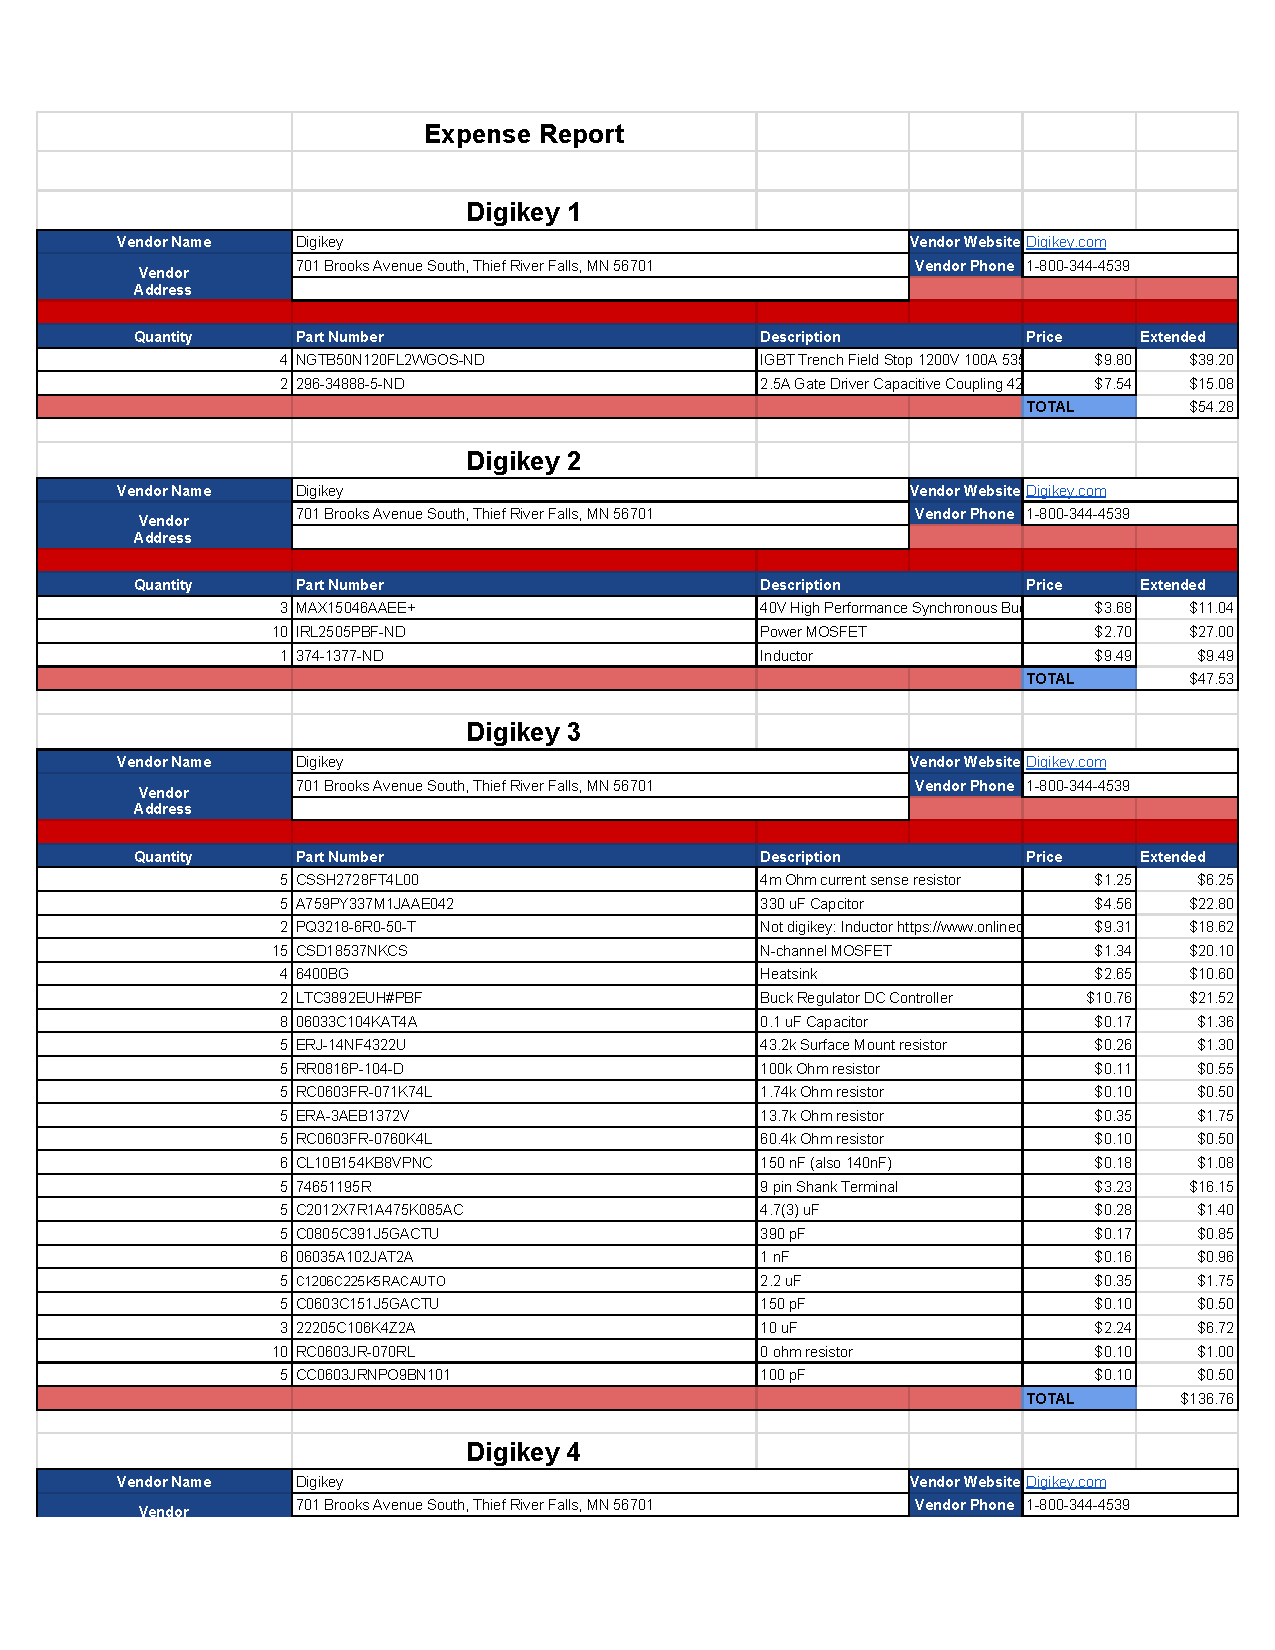
\includegraphics[width=1\textwidth]{ExpenseReport.pdf}
\end{figure}

\newpage

\section{Appendix: Datasheets}

\subsection{LM2575 Buck Converter}

\begin{figure}[H]
    \centering
    \includegraphics[width=1\textwidth]{buck1.JPG}
\end{figure}

\begin{figure}[H]
    \centering
    \includegraphics[width=1\textwidth]{buck2.JPG}
\end{figure}

\newpage

%\subsection{TMP36 Temperature Sensor}

%\begin{figure}[H]
    %\centering
    %\includegraphics[width=1\textwidth]{tmp1.JPG}
%\end{figure}

%\begin{figure}[H]
    %\centering
    %\includegraphics[width=1\textwidth]{tmp2.JPG}
%\end{figure}

\subsection{LT1336 Half-Bridge N-channel Power MOSFET Gate Driver}

\begin{figure}[H]
    \centering
    \includegraphics[width=1\textwidth]{LT1336.pdf}
\end{figure}

\begin{figure}[H]
    \centering
    \includegraphics[width=1\textwidth]{driver1.JPG}
\end{figure}

\newpage

%\includepdf[pages={1,2}]{LT1336.pdf}

\subsection{FDP8447L N-channel PowerTrench MOSFET}

\begin{figure}[H]
    \centering
    \includegraphics[width=1\textwidth]{mos.JPG}
\end{figure}

%\subsection{CP603333 Peltier Device}

%\includepdf[pages={2,5}]{Peltier.pdf}

\section{Appendix: Operating Instructions}

To operate device:\newline
1. Plug device into 120V outlet. \newline
2. Place lid on the chamber to withhold temperature \newline
3. Set desired temperature with Discovery Board joystick. \newline
Up Button: +1$\degree$C \newline
Down Button    -1$\degree$C\newline
Center Button  -10$\degree$C\newline
Right Button:	  +10$\degree$C

\end{document}